%---------------------------------------------------------------------------------------------------
% Francisco Gimenez
% December, 2015
% PhD Dissertation
% Stanford University, Program in Biomedical Informatics
%
%---------------------------------------------------------------------------------------------------

%---------------------------------------------------------------------------------------------------
% Packages

\documentclass[12pt,twoside]{report}		% double-sided for binding. font size: 10, 11, or 12 pt.
\usepackage{suthesis-2e-poznik}             % Stanford Dissertation .sty file, with my edits
\usepackage{amsmath}						% mathematical formulas
\usepackage{amssymb}						% mathematical symbols
\usepackage{graphicx}						% \includegraphics for eps and pdf graphics
\usepackage{cite}							% to clean up citations in the main text
\usepackage[labelfont=bf,labelsep=period]{caption}	% bold figure number in caption
\usepackage{subcaption}						% for subfigures
\usepackage{color}							% to color text: {\color{red} text}
\usepackage[usenames,dvipsnames]{xcolor}	% more flexibility for colors
\usepackage{amsfonts}						% \mathcal, \mathbb, \mathscr, etc
\usepackage{amsthm}							% \newtheorem{name}{Printed output}
\usepackage{amscd}							% rectangular diagrams
\usepackage{verbatim}						% reproduce every char w/in \begin{verbatim} ... 
\usepackage{epstopdf}						% convert eps to pdf
\usepackage[backref]{hyperref}				% hyperlinks; backrefs in bibliography
\usepackage[nameinlink,noabbrev]{cleveref}  % capitalize at start of sentence
\usepackage{setspace}						% for line-spacing
\usepackage{fancyhdr}						% enables fine control over headers and footers
\usepackage[super]{nth}						% for super-scripting 1st, 2nd, etc.
\usepackage{courier}    					% sets \ttfamily to courier new
\usepackage{rotating}						% for rotating figures and captions
\usepackage{afterpage}						% for placement of rotated figures and captions
\usepackage{booktabs}						% to make book-quality tables
\usepackage{bm}								% enables boldface in math mode with \boldsymbol{}
\usepackage{tabularx}						% word wrapping in tables
\usepackage{multirow}						% enables spanning multiple rows in a table
\usepackage{float}							% enables H to force figure placement here
\usepackage[T1]{fontenc}					% modern font encoding
\usepackage{lmodern}						% latin modern font
\usepackage{algorithm}						% algorithm float box
\usepackage{algpseudocode}					% algorithmicx type setting
\usepackage{apacite}						% apa style (author year)

%---------------------------------------------------------------------------------------------------
% updates to algorithmic package
\renewcommand{\algorithmicrequire}{\textbf{Input:}}  % \require = INPUT:
\renewcommand{\algorithmicensure}{\textbf{Output:}}  % \ensure = OUTPUT:
\newcommand*\Let[2]{\State #1 $\gets$ #2}  %\LET{a}{b} = a \gets b


%---------------------------------------------------------------------------------------------------
% Math operators to for argmax and argmin
\DeclareMathOperator*{\argmax}{argmax}
\DeclareMathOperator*{\argmin}{argmin}
%---------------------------------------------------------------------------------------------------
% Specify my figures folder
\graphicspath{{./figures/}}
%---------------------------------------------------------------------------------------------------
% Electronic submission:
% * Set \onlinetrue: removes copyright and signature pages
% 
% Actual dissertation:
% * Comment out \proposaltrue
% 	a. removes "proposal" from title page
% 	b. includes acknowledgments
% * Comment out proposed work chapter and uncomment discussion chapter.

%\proposaltrue								% affects title page, acknowledgements, final chapter
%\onlinetrue								% electronic submission: remove copyright and signature pages

%---------------------------------------------------------------------------------------------------
% Includeonlies. To compile a shorter list of .tex files.

%\includeonly{abstract,preface,chapter1-introduction}

%---------------------------------------------------------------------------------------------------
% Bibliography

% bibliography style
%\bibliographystyle{unsrt}					% bibtex style. e.g., plain (sorted), unsrt, plos2009
\bibliographystyle{apacite}
%\makeatletter								% enables usage of @ in package modification
%\renewcommand{\@biblabel}[1]{\quad#1.}		% remove brackets from numbering in list of references
%\makeatother								% returns @ to normal usage
%\renewcommand*{\backref}[1]{[#1]}			% format back references in bibliography

%---------------------------------------------------------------------------------------------------
% Settings

% hyperlinks
\definecolor{linkCol}{RGB}{23,118,153}		% yields plos genetics color: 23,98,135
\hypersetup{
    colorlinks,								% colors text rather than surrounding it by a box
    linkcolor={linkCol},					% internal links
    citecolor={blue!50!black},				% citations: 50% blue, 50% black
    urlcolor={blue!80!black}				% web links and urls: 80% blue, 20% black
}

%---------------------------------------------------------------------------------------------------
% Title Data

\title{Fast adaptive structured reporting for decision support in radiology}
\author{Francisco J. Gim\'{e}nez}
\programthesis
\dept{Biomedical Informatics}
\principaladviser{Daniel Rubin}
\firstreader{Ross Shachter}
\secondreader{Mark Musen}

%---------------------------------------------------------------------------------------------------
% Start Document

\begin{document}
\beforepreface						% title, copyright, and signature pages

%---------------------------------------------------------------------------------------------------
% Prefaces. Each must begin with: \prefacesection{myTitle}.

\prefacesection{Abstract}
Radiology is a powerful tool to detect and diagnose abnormalities by allowing doctors to visually inspect internal pathology that could not otherwise be seen. However, assessing radiological images is limited by variations among practitioners, including deficiencies in their reporting of these imaging examinations as well as in their interpretations. Three main sources of these variations in interpretation are incorrectness of observations in the images, incompleteness of the radiological observations reported to characterize the abnormalities, and inconsistency of these observations with respect to the radiologists' overall impression. We hypothesize that the quantification and enforcement of correctness, completeness, and consistency of radiological observations will improve the diagnostic accuracy and reduce variability of interpretation. To test this hypothesis, we propose a decision support system that provides feedback to radiologists during the reporting of their radiological observations. We will develop this system by creating novel statistical models to link radiological observations, computational imaging features, and disease to recognize incorrectness, incompleteness and inconsistency in reporting. We will then harness these models to create a quantifiable metric of observation quality. We propose a research plan with the following specific aims: (1) To characterize breast lesions seen in mammography images by capturing computationally-derived (``quantitative'') imaging features and radiologist-derived observational (``semantic'') features, (2) develop metrics to measure incorrectness, incompleteness, and inconsistency, and (3) develop a decision-support system to improve these metrics. We will test this system in mammography, and show how it can be extended to other imaging domains and possibly to other medical domains where diagnostic reasoning is documented in dictated reports.


\ifproposal 						% exclude acknowledgements from proposal
\else 
	\prefacesection{Acknowledgements}
If this dissertation was 100 times longer, I still would not be able to hand out a souvenir page to all the amazing people in my life who have helped me along the way. That being said, I want to make explicit the gratitude I show to several of my friends and mentors.

To my advisor Daniel Rubin, you have been exactly everything I needed to do this work. You gave me enough freedom to grow as a research on my own while still providing enough guidance such that I didn't get lost in the purgatory of aimless projects. Whatever skills and success I have as a scientist are due in large part to how you showed me how to think.

To my committee members Ross Shachter, Mark Musen, and Curt Langlotz, thank you for the extremely entertaining and enlightening conversations. Ross, you challenged me like no other and always caught my mistakes in reasoning. It has made your approval so much more worthwhile. Mark, I would often find myself floating around MSOB looking to talk shop, and you would always indulge me if you had the time. It was always worth stopping by to talk about research and life in general. Curt, I am pretty annoyed you took so long to come to Stanford given how helpful you have been to me in the past year and half. I don't think I could ever approach being as smart as you, but I'll sure as hell try.

To BMI faculty and staff, you made the program feel more like a family than graduate school. Thank you MaryJeanne Oliva, Nancy Lennartson, John DiMario, Russ Altman, Nigam Shah, Dennis Wall, and David Paik. Stanford seemed like an intimidated place to go to graduate school until I met you all and felt welcomed.

To the Bankiewicz lab, especially Krys, John, Piotr, Mishek, and old Francisco. You taught me that research was my calling and were one of the biggest influences on my future. Thanks for taking a chance on my 20 year old self however annoying I may have been.

To my outstanding high school teachers, you taught me to love learning. Mr. Tastor, Mr. Fisher, Mrs. Kars, Mr. Westberg, whatever seed you planted in me remained today (for better or for worse).

To my BMI colleagues, you have been the best peers, friends, therapists, and guardians. Brian you were a great roommate, friend, and surfing buddy and are likely one of the funniest people I know. Jonathan, I thought you were extremely weird when I first met you, and I haven't really changed my mind about that, but you have come to be such a wonderful partner in crime. Beth, it has been a pleasure learning about life with you on our frequent coffees and beers. Katie, you always keep me on a tight leash, but you are easily the most dependable friend anybody could have. Diego, thanks for being my video game sherpa and carrying so hard. Pablo, we formed a Latino czar dream team that will never be beaten. Moskowitz, your love of food and sense of humor pretty much means I will always make time to hang out with you. Dpoz, you are easily one of the most dedicated and honest people I know, and I will always secretly try emulate that. Sarah, thank you so much for being an acceptor of all things weird; I wish you stayed around us a little longer. There are likely a lot of you I missed, take this section as an opportunity to call me out on it and I'll buy you a beer.

To Mom, Dad, Alfredo, Ari, and Lisa, you are the best family I could have. I know no better times than spending time with you all, and hard times have been a breeze knowing you were there for me. I am forever indebted and hope I give you a fraction of the support, joy, comfort, and love you have given me.

Finally, I would like to thank my funding sources the National Library of Medicine Training Grant (LM007033) and the National Institutes of Health for my Ruth L. Kirchstein National Research Service Award Fellowship (1F31CA171789-01A1 ).  
\fi	

%---------------------------------------------------------------------------------------------------
% Post-Preface Front Matter

{ \hypersetup{hidelinks}			% keep TOC black
  \contentstablesfigures }			% tables of contents, tables, and figures
\startmaindoc						% start main body: \cleardoublepage, arabic page 1, headings

%---------------------------------------------------------------------------------------------------
% Chapters. Each must begin with: \chapter{myChapterTitle}.

%\import{text/}{intro_chapter}
%\import{text/}{radiology}
%%\import{text/}{decision_support}
%\import{text/}{annotation_verification}
%\import{text/}{completeness_analysis}
%\import{text/}{feedback}
%\import{text/}{conclusions}

\chapter{Introduction}
Radiology is a powerful tool to detect and diagnose abnormalities by allowing doctors to visually inspect internal pathology that could not otherwise be seen. Though it is an indispensable part of the diagnostic workup, the practice of radiology is still fraught with error due to the inherently subjective nature of the task; the doctor must still visually scan, detect, and interpret the findings in the image to deliver an impression. An unfortunate consequence of such a system is substantial variability in practice and performance. This dissertation aims to tackle these shortcomings. To do so, I propose a novel computational decision-support paradigm aimed at improving the quality and content of the radiological \emph{report} rather than the traditional approaches aimed at directly improving the diagnosis. I develop informatics methods within this paradigm to detect and reduce error in reports, and show how these methods have the potential to improve overall diagnostic performance. This chapter provides an overview of the dissertation. I begin by providing a brief background of radiological error, decision-support systems, and reporting. I then give a high-level description of my proposed decision-support model, methods, and key results. Finally, I delineate my contributions to the field and provide a guide to the reader for the remainder of the document.

\section{Radiology, variability, and errors}
Radiology is an essential part of modern clinical medicine, constituting 10.6\% of health care spending and is virtually ubiquitous in every part of health care \cite{Dodoo:tg}. The field has traditionally been at the forefront of medical technology by virtue of its foundations and reliance upon sophisticated technological achievements. Digital radiology and picture archiving and communications systems led to an early, widespread adoption of electronic records with respect to imaging \cite{Strickland:2000cv,Bryan:1999kn}. But, despite the early adoption of computational systems to manage data, the actual practice of radiology remains a relatively unchanged. An unfortunate consequence of such a system is substantial variability in practice and performance \cite{Fitzgerald:2001hn}. \citeA{Robinson:1997uq} went so far as to state that ``errors and variations in interpretation now represent the weakest aspect of clinical imaging'' and declared such issues as ``Radiology's Achilles' heel''. This is not to say that radiologists are the only doctors faced with these issues, as the now infamous Institute of Medicine report \emph{To Err is Human: Building a Safer Health System} revealed a striking amount of poor patient outcomes are a result of medical error \cite{Anonymous:2000va}. A prominent recommendation from this study is the use of automation and computation to improve upon standard of care via decision support systems.

\section{Radiological decision-support}
Decision support systems are tools that incorporate medical information to provide meaningful input to medical practitioners. The main source of medical information in radiology is confined to patient history drawn from the electronic medical record, the patient images, and the reports generated by the radiologists. As a result, it is a ripe domain for decision support tools to assist in organizing, analyzing, and synthesizing these data sources. 

Radiological data mining allows clinicians to query similar cases to the ones they are evaluating \cite{Shin:2015wl,Bozkurt:2014jw,Depeursinge:2012ce,Korenblum:2011gx,Akgul:2011ey,Nassif:2009du}. Computer-aided detection (CADe) systems assist in identifying abnormalities in images across a variety of radiological domains such as mammography, colonoscopy, lung screening, and liver diagnosis \cite{Cheng:2003ig,Castellino:2005ke,Meeuwis:2010bv,Oliver:2010fm,Fenton:2011fw,Fenton:2012kz,Jamieson:2012hz,Gallas:2012eg,Giger:2013jb}. Computer-aided diagnosis (CADx) systems assist in interpretation of abnormalities found in the image \cite{Jiang:1999fj,ElizabethS:2005gc,Gallas:2012eg,Bright:2012ga,Giger:2013jb,Depeursinge:2010jl,Fujita:2008it,Eadie:2011cv,Rubin:2005jg,Garg:2005cb,Elter:2009fv,Jamieson:2010vl,Jamieson:2010tt,Cheng:2003ig,Jiang:2001fy} as well as interpretation of the content within the radiology report \cite{Burnside:2000wl,ElizabethS:2005gc,Burnside:2009br,Rubin:2005jg}.

Despite significant technological achievements, adoption of these systems in radiology is limited. In particular, the only commercially deployed radiological decision support systems are computer-aided detection (CADe). The main reasons for this inability to affect practice is that these systems often interrupt clinical  work-flow, give assessments rather than recommendations, and fail to provide decision-support during decision-making \cite{Kawamoto:2005gn,Morgan:2011ct}. These shortcomings are not unique to radiological decision support; they exhibit the same symptoms of decision support systems in other clinical domains that did not see commercial adoption. In general, they still follow the the so-called \emph{Greek Oracle} model of decision support \cite{Miller:1990wg,Miller:1994cx}. Such systems fail when deployed in practice since they are based on the implicit assumption that computers can perform the duties of doctors better than doctors themselves. Charles Friedman goes so far as to declare that the \emph{Fundamental Theorem of Biomedical Informatics} is that decision support should ``augment human reasoning'' beyond the capabilities of an unaided practitioner \cite{Friedman:2009dx}. Thus, it is crucial to develop radiological decision support tools that fit into the work-flow and augment their reasoning. A perfect window to provide this is during radiological reporting.

\section{Radiology reporting}
The radiology report conveys the radiologist's findings, interpretation of these findings, and suggested patient management. It is also the primary form of communication of this information to referring clinicians or patients \cite{Sistrom:2005cx}. Given that communication breakdowns constitute 80\% of medical malpractice lawsuits \cite{Levinson:1994ko}, and radiological reports are legally admissible court documents \cite{Oppenheim:2012tq}, considerable effort has been made to measure and improve upon report quality \cite{Langlotz:2015vq}. These studies have identified key tenets of report quality: correctness of findings, completeness of the description of significant clinical findings, consistency of report language and findings, and timeliness of the report's completion \cite{Johnson:2004kh, HaraldO:2004hi, Reiner:2006fa}. 

Several projects aim to improve the quality of radiology reports. Standardization of mammography reporting via the Breast Imaging Reporting and Data System (BI-RADS) has led to uniform reporting language and assessment guidelines \cite{Liberman:ws,Langlotz:2009fn,Burnside:2009ki}. RadLex is an effort to extend standardization of terminology by defining a lexicon of all radiological concepts \cite{Langlotz:2006jn}. In addition to terminology, there is a strong push to create \emph{structured reports} that further standardize report format and organization \cite{Langlotz:2009dd,Reiner:2009ib}. Structured reports not only can improve communication, but they allow for computability of the report information beyond the constraints of free-text documents. Unfortunately, structured reporting is not without its drawbacks. It requires new software to implement into the clinical work flow which is costly in terms of implementation and training. More importantly, structured report creation is time-intensive and imposes distractions in the traditional radiological work flow, directly interfering with timeliness \cite{Weiss:2008er}. Despite these shortcomings, structured reporting is widely seen as the future of radiological reporting \cite{Langlotz:2015vq}.

Both standardized terminology and structured reports are solid steps to improving upon the reporting process, but they do not directly analyze the radiological concepts being communicated. Borrowing from the \emph{meaning triangle}, the tools described encode radiological objects with standard expressions, but they do not encode their sense or concept \cite{Mead:2006wm}. Such work would need to perform higher order analysis of the information in the report including, but not limited to, analyzing if the contents in the reports is correct, complete, or even consistent with diagnosis. In this sense, decision support systems provide the missing piece for this analysis.

\section{Providing decision support during reporting time}

My hypothesis is that delivering decision support during reporting time to improve completeness and correctness of reports will improve consistency, and therefore, diagnostic performance. To this end, I seek to answer the following questions:

\paragraph{How can we improve the quality of radiological report?}

Though I have described methods to improve the terminology and format of the report, there is much to be done to improve upon the \emph{content} of the report. What can we do to improve upon this information? How can we actually implement such solutions?

\paragraph{Does improving the report improve diagnostic performance?}

There are no studies showing that improving the content of the radiological report can actually improve the diagnostic performance of the physician. If we implement new methods to improve the report, will they have any effect on the radiologist's outcome? Otherwise, are we needlessly burdening radiologists with technology to fix reporting for its own sake?

\subsection{Specific Aims}

\begin{enumerate}
	\item Develop methods to assess completeness and correctness of radiology reports
	\item Evaluate these methods in two important radiological domains (mammography and liver CT)
	\item Use completeness and correctness metrics to provide feedback to improve consistency and diagnostic performance
\end{enumerate}

\subsection{Methodology}

\begin{figure}[h]
	\centering
	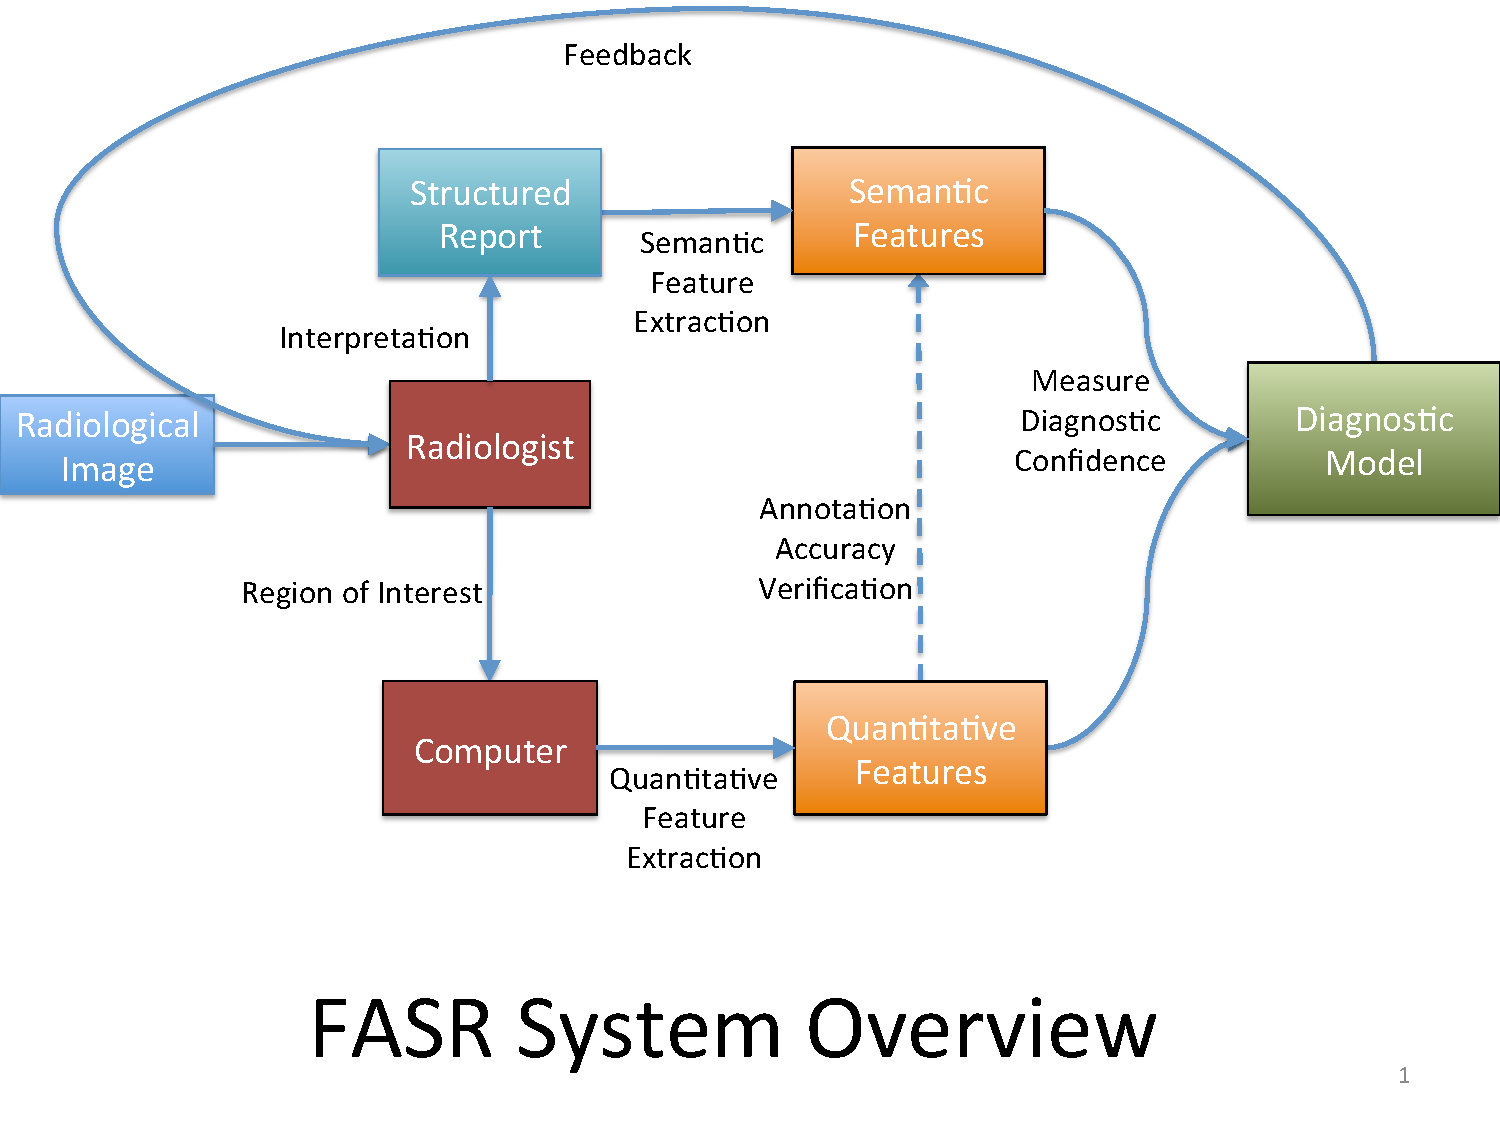
\includegraphics[width=1\linewidth]{fasr_diagram.pdf}
	\caption{Overview of the Fast Adaptive Structured Reporting (FASR) system}
	\label{fig:fasr_diagram}
\end{figure}

To tackle this challenge and to enable translation of decision-support system into clinical practice to benefit patient care, I propose a real-time decision-support system that provides feedback to radiologists as they generate their reports called Fast Adaptive Structured Reporting (FASR). This system will create evaluate and improve upon the content of a structured radiological report. This differs from traditional approaches to decision-support system because our system will improve upon reporting, and by our hypothesis, implicitly improve upon practice. By ensuring that the relevant observations are correctly, completely, and consistently described in mammography reports, our decision-support system will reduce variability in practice, improving practitioner decision making and lead to better patient care.

\subsection{Key Results}


\section{Summary of contributions}
This work demonstrates contributions to the our understanding of reporting in radiology as well as performance of decision-support systems for diagnostics.

\subsection{Radiology contributions}
\subsubsection{Automatic annotation and verification of descriptors in liver CT scans}
\subsubsection{Correlated incomplete reports with diagnostic error}

\subsection{Informatics Contributions}
\subsubsection{General purpose semantic classification of images}
\subsubsection{Monte-Carlo computation of same-decision probability}
\subsubsection{Framework for delivering and evaluating feedback in decision-support systems}


\section{Guide for the reader}

\chapter{Radiology}
In this chapter I provide background into the problems and current solutions to decision support in radiological reporting. I begin by describing the clinical applications that I study throughout this text: liver imaging and breast imaging. I then describe some of the large issues in clinical radiology with respect to these domains. Finally, I describe decision support systems within these two domains, their contributions to the field, and shortcomings that I address in my works.


%\section{Radiological image interpretation and reporting}
%\subimport{text}{radiography_background}
\clearpage
\section{Clinical applications}
Radiology touches upon nearly every part of medicine that concerns abnormalities within the human body. In this work, I focus upon two major domains for applications: liver imaging and breast imaging.

\subsection{Liver imaging}
Liver lesions stem from a variety of causes, both cancerous and non-cancerous. Imaging of the liver is the primary method to differentiate lesions efficiently and accurately in a non-invasive manner. In particular, hepatocellular carcinoma (HCC) is a particularly important cancer to detect early as it is the fifth most common cancer and the third most common cause of cancer-related deaths \cite{Willatt:2008gs}. Screening and surveillance efforts have led to more prominent usage of liver imaging to diagnose such cancers.

\paragraph{Contrast-enhanced CT of the liver}
Contrast-enhanced CT imaging is the dominant technology used for liver lesion diagnosis \cite{Baron:1994vg}. This modality takes advantage of the fact that the liver receives blood from two main sources, the portal vein and the hepatic artery. The portal vein supplies about 80\% of blood to the liver with the hepatic artery providing the other 20\%. Due to varying physiology among liver lesions, differing lesion types may not share the same blood intake proportions as the surrounding liver tissue. Multi-phasic contrast-enhanced imaging takes advantage of this by obtaining images of the liver at multiple time points after injection of contrast agent. This allows for visualization of lesions due to the difference in time between the arrival of contrast agent in the hepatic and portal circulations. This difference causes several distinctive imaging features on contrast-enhanced imaging. As an example, primary liver cancer tumors receive most of their blood from the hepatic artery, so they contain higher concentrations of contrast agent than surrounding liver parenchyma during the arterial phase \cite{Lautt:1987wma,Matsui:1991vba}. Arterial-phase contrast-enhanced CT, therefore, may be helpful in finding masses that exhibit malignant tumor characteristics. Other phases may be useful for differentiating tumor types. For example, metastatic tumors appear less dense compared to the normal liver during the portal venous phase.

The difference in density between a lesion and its surrounding tissue at various times after the injection of iodine in a peripheral vein in multi-phasic imaging is called the temporal enhancement pattern. Analysis of a lesion's temporal enhancement pattern through the different phases of image acquisition helps radiologists to make diagnoses. Unfortunately, the specificity of this method is a function of the size of the lesion and prone to a high false positive rate because several types of liver lesions, including benign ones, have similar manifestations on CT images \cite{Lencioni:2005ia}.

\subsection{Breast imaging}
Breast cancer affects 1 in 8 women in the United States. It is the second leading cause of cancer deaths amongst women \cite{Siegel:2012kt}. Early detection has been shown to reduce the mortality of cancer by catching the disease while it is more easily treatable \cite{Baker:1982jg}. Mammography was developed in an effort to improve such early detection.

\subsubsection{Mammography screening and diagnosis}
Mammography is the use of x-ray imaging on the breast to identify any abnormalities. Radiologists presented with mammograms are tasked with two problems: detection and interpretation. Detection is the task of visually inspecting the mammogram and locating any possible abnormalities. Interpretation is evaluating whether detected abnormalities are suspicious for breast cancer.

Mammography has shown to be beneficial for early detection of breast cancer \cite{Nystrom:2002hb}. Currently, the American Cancer Society recommends that women with no specific risk for breast cancer get yearly screening mammograms to catch potentially malignant findings early \cite{Smith:2003en}.

\subsubsection{Interpretation of mammography findings}
Formally, the interpretation problem is defined as follows: A radiologist is presented with a lesion in a mammogram, patient history and demographics, and possibly prior mammograms. The radiologist must decide whether this lesion warrants no action or follow-up (either imaging or biopsy) based on their suspicion of malignancy. This suspicion of malignancy is quantified as the BI-RADS assessment category, which is an ordinal value ranging from 1 to 6. An additional assessment category of 0 is used to indicate there is not enough information in the mammogram to make a decision. These assessment categories were designed to have probabilistic interpretations, where each value has a range of posterior probabilities of malignancy as shown in Table \ref{table:birads}. A BI-RADS assessment of 1, 2, or 3 indicates the recommendation is no immediate follow-up (a negative assessment). A BI-RADS assessment of 4 or 5 indicates a recommendation for follow-up imaging or biopsy should be considered (a positive assessment). An assessment of 0 should not count as either positive or negative, but the fact that it necessitates immediate follow-up imaging means that it is treated as a positive finding \cite{Barlow:2004cy}. BI-RADS 6 is a non-diagnositc category used to indicate that the images reflect a known cancer diagnosis being evaluated for treatment planning. These assessment categories implicitly mean that any lesion with a posterior probability of greater than 2\% should be considered as a positive finding. Recent work has shown that this 2\% threshold rule is justified via epidemiological risk analysis \cite{Burnside:2012fk}. In addition to providing an assessment, radiologists must provide a report that justifies their decision. This report has a set of categorical descriptors standardized by BI-RADS, which can be interpreted as evidence for their decision.

\footnote{The description provided here is with relation to the 4th edition of BI-RADS, which was released in 2003. The 5th edition (released in 2013) of BI-RADS has altered the names of several descriptors and recommendations for assessment categories. Because all the mammography data used for analysis was collected before the release of the 5th edition, we will work under the framework of the 4th edition. All the methods described can easily be extended to adopt the conventions of the 5th edition.}

\begin{table}[ht!]
\centering
\begin{tabular}{|c|c|c|}
	\hline  BI-RADS Assessment&  Probability of Malignancy & Description \\ 
	\hline\hline
	0& N/A & Additional Imaging Needed \\ 
	\hline
	1& 0\% & No Abnormality \\ 
	\hline  
	2& 0\% & Benign Finding  \\ 
	\hline  
	3& $<$ 2\% & Probably Benign Finding \\ 
	\hline  
	4& 2-95\% & Suspicious Abnormality \\ 
	\hline  
	5& $>$ 95\% & Highly Suggestive of Malignancy \\ 
	\hline  
	6& 100\% & Biopsy Proven \\ 
	\hline 
\end{tabular}
\caption{The BI-RADS assessment categories and their probabilistic interpretations.}
\label{table:birads}
\end{table}


\subsubsection{Mammography screening controversy}
The American Cancer Society recommends annual screening mammography for women over 40 to detect breast cancer early when it is most treatable \cite{Nystrom:2002hb, Smith:2003en, Smart:1997hk}. However, this recommendation has been refuted by several longevity studies \cite{Bleyer:2012dc, Kalager:2012ez},  culminating in the United States Preventative Services Task Force recommending biennial screening after 50 years of age \cite{Kerlikowske:2013ej, Anonymous:2009fl}, which argues that unnecessarily early and frequent screening results in high economic and emotional costs. While a reduction in screening is one possible solution to addressing the issue of erroneous detections, it comes at the cost of possibly missing cancer at an early stage. An alternative solution is to directly improve radiologist performance.


\clearpage
\section{Error and variability}
Errors in the interpretation and diagnosis in radiology are well-known shortcomings in radiology \cite{Fitzgerald:2001hn}. The nature of the field requires that humans provide a subjective assessment of medical images and make medical decisions under such uncertainty \cite{Wood:1999ew}. Such a model of practice leads to error and variability in performance. In this section, I review some of the prevalent studies measuring this error.

\subsection{Error in interpretation of liver CT}
Recent efforts to screen at-risk populations for hepatocellular carcinoma spurred studies into performance of diagnosis. \citeA{Brancatelli:2003tm} studied the false positive rate of helical CT imaging, finding an 8\% false positive rate in a population of 1,329 patients. False negatives are also a an issue when lesions are small (< 2cm) due to their difficulty in detection and interpretation \cite{Willatt:2008gs,Lencioni:2005ia}. CT scans are costly procedures that expose users to non-trivial amounts of radiation. As a result, their usage to screen patients needs to be justifiable with respect to diagnostic accuracy. These errors constitute a major obstacle in preventive screening for at-risk patients.

\subsection{Error in interpretation of mammograms}
Mammography is one of the most common imaging tests performed today, and as a result, there is substantial literature documenting its error and variability. Much of this is inherent to the nature of screenings exams. Like all screening tests, mammography trades off sensitivity with specificity. These trade-offs are determined by a radiologists' personal model of practice, which is subjective. A conservative radiologist might practice at an increased sensitivity, meaning fewer false negative findings, at the cost of reduced specificity, meaning more false positives. Such subjectivity results in variability in mammography practice. 

A review by \citeA{Boyer:2012gk} analyzed the sources of error mammography interpretation. They found two types of reading errors (quoted from the review):

\begin{enumerate}
	\item ``Detection errors occur when a lesion is not seen by the reader. Missed lesions tend to occur in dense breasts, are often present as a mass and are frequently found in the retroglandular area.
	
	\item ``Interpretation errors'' occur when the lesion is detected but misinterpreted by the reader.
\end{enumerate}

In this work we focus on interpretation errors.

\subsubsection{False positive errors in mammography}
The driving factor behind actual errors in mammography reading is false positive findings \cite{Kerlikowske:2013ej}. This is due in large part to the fact that breast cancer is a low probability event, so false positive findings are much more likely to occur in volume than false negatives. Furthermore, mammography is designed to be extremely sensitive to breast cancer, leading to conservative practice standards so as not to miss potential cancers. Though a false negative finding has the obvious negative impact in that it delays treatment, false positive findings are a growing concern. Not only do they lead to unnecessary and costly testing, but they cause long term psychosocial harm in patients \cite{Brett:2005gq,Brodersen:2013kq}.


\subsubsection{Individual radiologist variability in diagnosis}
The primary method to quantify radiologist performance in mammography is with receiver-operating characteristic curve analysis. \citeA{Beam:1996ui} was the first to document significant variability in mammography, showing a range of 40\% in sensitivity and a range of 11\% in overall accuracy.\citeA{Barlow:2004cy} performed a systemic analysis of a large cohort of radiologists, revealing significant variability in sensitivity and specificity of diagnosis [Figure \ref{fig:barlow_variability}]. He measured the performance of 124 radiologists over a 5-year period and found their recall rates ranged from 1.8\% to 26.2\% , specificity ranged from 74\% to 98\% , and sensitivity ranges were not reported due to being extremely large as a result of few true cancers. They tested for variability between these performance values and all were deemed significant. \citeA{Elmore:2009vu} replicated these studies with 187 interpreting 1,036,155 screening mammograms in 531,705 women [Figure \ref{fig:elmore_variability}]. She found that ``interpretive performance varied widely with the median and interquartile ranges for performance measures as follows: recall rate, 9.3\% and 6.3\%-13.2\%; false-positive rate, 8.9\% and 5.9\%-12.8\%; sensitivity, 83.8\% and 74.5\%-92.3\%; and PPV1, 4.0\% and 2.6\%-5.9\%, respectively.''

\begin{figure}[h!]
	\centering
	\includegraphics[width=1\linewidth]{barlow_variability.pdf}
	\caption[ROC analysis of 124 radiologists over a 5 year screening period]{ROC analysis of 124 radiologists over a 5 year screening period. Radiologists viewed 469,512 mammograms which were linked to cancer outcomes. Variability in sensitivity and specificity of radiologists was found to be statistically significant}
	\label{fig:barlow_variability}
\end{figure}

\begin{figure}[h!]
	\centering
	\includegraphics[width=1\linewidth]{elmore_variability.pdf}
	\caption[Performance of 187 U.S. radiologists who interpreted images from screening mammographic examinations]{Performance of 187 U.S. radiologists who interpreted images from screening mammographic examinations (with images from one or more examinations associated with a cancer diagnosis). Sensitivity and false-positive rate are shown for each radiologist. Specificity was calculated by subtracting false-positive rate from one. Size of circle represents number of screening mammograms interpreted by that radiologist that were associated with a cancer diagnosis, with larger circles representing more cancers. Small circle may represent a radiologist with screening mammograms associated with one or two cancers. Normalized partial area under the curve is 0.82. Two areas are in color to highlight radiologists with both sensitivity and false-positive rate in highest (>75th percentile in green) and lowest (<25th percentile in red) rating for interpretive performance on basis of national BCSC benchmarks for screening performance (11). Figure and caption from \cite{Elmore:2009vu}}
	\label{fig:elmore_variability}
\end{figure}



\subsubsection{Institutional diagnostic variability in mammography}
Beyond individual radiologist variability, \citeA{Taplin:2008bv} showed that \emph{institutions} have significant variability in their specificity, $PPV_1$ and $PPV_2$ (though no statistical significance was shown in sensitivity, likely due to the inherent variance in sensitivity for mammography) [Figure \ref{fig:taplin_variability}].

\begin{figure}[h!]
	\centering
	\includegraphics[width=1\linewidth]{taplin_ppv_variability}
	\caption[Institutional variability in mammography]{Screening mammography performance measures for the 44 facilities. A) Sensitivity. B) Specificity. C) Positive predictive value of any additional evaluation ($PPV_1$). D) PPV of referral for biopsy ($PPV_2$). Diamonds indicate mean values; error bars correspond to 95\% confidence intervals. The 44 facilities varied statistically significantly in specificity (P < .001), $PPV_1$ (P < .001), and $PPV_2$ (P = .002) but not in sensitivity (P = .99). Figure and caption from \cite{Taplin:2008bv}}
	\label{fig:taplin_variability}
\end{figure}


\subsubsection{Radiologist variability in BI-RADS usage}
Although BI-RADS to standardizes the terminology in mammography reports, it cannot fully enforce how these terms are used. \citeA{Liberman:ws} first showed hints that variability is a problem in usage of descriptors. They had five radiologists evaluate 60 of the same mammography studies and found considerable disagreement in ``associated findings'' and ``special cases.'' A similar study by \citeA{Berg:2000jf} had five mammographers evaluate 103 screening mammograms and they saw significant variability in usage of descriptors as well as BI-RADS assessments. They did a follow up study that showed how this could be reduced by specific BI-RADS training, but the system only helped for evaluation of masses \cite{Berg:2002fy}. \citeA{Lazarus:2006bl} performed a study solely focused on descriptor agreement between five radiologists in 94 cases. They found similar results with moderate agreement of mass descriptors and less agreement with calcification descriptors. All kappa values in for mammography were below 0.5 in any descriptor.





%\section{Radiology reporting}
%\subimport{text}{reporting_background}
%\clearpage
\clearpage
\section{Decision support}
\subsection{Decision support for liver lesions}
Recent research has investigated computer-aided methods to support diagnosis by providing a database of annotated images that can be retrieved by similarity\cite{Napel:2010es} and further indicates that radiological observations drawn from a controlled vocabulary can lead to accurate diagnoses of liver tumor types from CT images\cite{Korenblum:2011gx}. These observations can be treated as features of the image derived from human semantic annotations. As a result, we refer to them as semantic features. These semantic features allow radiologists to make their observations consistent, explicit, and machine-accessible. Radiological tools such as the ePAD \cite{Rubin:2008uz} have been implemented with the purpose of recording these annotations in a facile manner.

Computational analysis of these images may overcome this issue by creating quantitative and unbiased descriptors of image features. These computational features can be computed directly from the image's pixel values, independent of the semantic features. Digital image processing techniques have been used to extract features indicative of lesion attenuation, texture \cite{Strela:2002vq,Zhao:2005wb}, edge and shape \cite{Hong:2006ti,Manay:2006un,MRangayyan:2005td,Xu:2012bh}.


\subsection{Mammography decision support}
Decision-support in mammography is grouped into two classes, computer-aided detection (CADe) and computer-aided diagnosis (CADx). 

CADe is used to automatically identify regions of interest to guide the radiologist after they have initially viewed the image without help. The goal is to reduce false negatives in detection of malignant lesions. CADx aims to improve the interpretation of a finding after a radiologist has identified it. In mammography this traditionally means determining if a finding warrants follow-up in the form of additional imaging or biopsy. Currently, the FDA has cleared several CADe products for use in clinical practice but there has not been as much success for CADx outside of academic research \cite{Castellino:2005ke, Oliver:2010fm, Fujita:2008it}. Though CADe continues to present interesting research, this thesis will focus on CADx.

In computational parlance, CADx problems are classification problems to predict state of malignancy of a finding given its features. Features of findings can be derived directly from the mammogram via computer vision and image processing techniques \cite{Jiang:1999fj,Jiang:2001fy, Giger:2013jb, Eadie:2011cv} or they can be derived from human observations \cite{ElizabethS:2005gc, Burnside:2000wl, Rubin:2005jg}. We refer to these as computational features and semantic features, respectively. Computational features have the advantage that they can be quickly and reproducibly extracted from the image. Semantic features, due to their subjective human readers, are much more variable and noisy. Despite these shortcomings, semantic features present much higher level information about the image and can incorporate the wealth of prior knowledge by the readers \cite{Liberman:ws,Elter:2009fv}.

Studies into deployment of medical decision-support systems help us understand why CADx systems have not seen adoption in clinical practice. Most CADx systems follow the Greek Oracle model of decision-support: they simply give an answer to the diagnostic task rather then assisting the radiologist to improve their own decision \cite{Miller:1990wg, Friedman:2009dx, Bright:2012ga}. Additionally, such systems interrupt the traditional radiological workflow \cite{Morgan:2011ct}. Despite these shortcomings, computer-aided diagnosis (CADx) could potentially diminish subjectivity in the interpretation of clinical information using quantitative methods and objective decision points. In addition, it would be possible to directly measure and tune performance in CADx systems; a task that is much more challenging in unassisted human readers. The difference between such systems and radiologists is that this tradeoff in CADx systems is explicitly set as the “operating point” (a particular value of sensitivity and the consequent specificity) on the receiver operating characteristic (ROC) curve of the system, which is used to assess and maximize the performance of CADx systems. In probabilistic CADx systems, a probabilistic threshold solely determines the operating point. This threshold can be interpreted as the minimum probability of cancer that a lesion must exhibit before it is deemed a positive finding (i.e. considered for biopsy). Most radiologists strive to have a fixed operating point, but given the qualitative nature of mammography interpretation, it is not possible for them to know their probabilistic threshold precisely. This is problematic since BI-RADS states that a probability of malignancy greater than 2\% should be considered a positive result \cite{Liberman:ws,Liberman:2002gg}; however, at present, there is no way to measure what threshold a radiologist is using. This makes it difficult to quantify if individual radiologists are practicing too conservatively by setting their threshold low to avoid missing cancers. While it is of utmost importance to detect cancer, an unnecessarily low threshold means more false positive detections. Even if a radiologist were deemed to be practicing too conservatively, it would be difficult to tune performance to practice less aversely.









%\import{text/}{decision_support}
\chapter{Verification of Radiologist Semantic Annotations}
\subimport{}{liver_intro}

\section{Annotating liver lesions via classification}
\subimport{}{liver_method}
\clearpage

\section{Experiment Design}
\subimport{}{liver_experiment_design}
\clearpage

\section{Results}
\subimport{}{liver_results}
\clearpage

\section{Lesion annotation prediction as verification}
\subimport{}{liver_discussion}
\chapter{Assessing Completeness of Radiological Reports}
Missing descriptors in mammography reports do not necessarily mean that the report does not have all the information to make a correct and justified diagnosis. Conversely, there are cases when most of the descriptors are reported, but the report still reaches an ambiguous diagnosis. Completeness of reports needs to be sensitive to the context of the information already given as well as the effect of missing information on the diagnosis. In this chapter I describe how to measure the information content of a radiological report. Information content being the value of the observations and descriptors in the report with respect to the diagnosis. I first describe a new metric to measure report completeness, then I propose an algorithm to compute this metric, and finally I perform a study that correlates report completeness with errors in radiological interpretation.
\clearpage

\section{Missing information in radiology reports}
Given that the final result of a mammogram is a decision whether to follow-up on patients with mammographic lesions, this decision should be the primary driver of determining whether enough information has been provided in the report. Early approaches to measuring whether medical diagnostic tests were necessary involved calculating thresholds for posterior probabilities that would warrant more testing or treatment \cite{Pauker:1980cg}. Such methods required that the practicing physician provide the posterior probability. The Pathfinder system used a value of information calculation to repeatedly request more information for diagnosis until there was only one possible diagnosis left \cite{Heckerman:1992uq}. This did not provide a flexible framework for stopping if there was more than one possible diagnosis outside of physician judgment. The STOP criteria provide a quantitative algorithm for when to stop requesting information and make a decision, but this is formulated only to measure whether the probability of an event exceeds a certain threshold \cite{Gaag:2011gs}.
\clearpage

\section{A metric to quantify incomplete reports}
Missing descriptors in mammography reports do not necessarily mean that the report does not have all the information to make a correct and justified diagnosis. Conversely, there are cases when most of the descriptors are reported, but the report still reaches an ambiguous diagnosis. Incompleteness of reports needs to be sensitive to the context of the information already given as well as the effect of missing information on the diagnosis. 

Given that the final result of a mammogram is a decision whether to follow-up on patients with mammographic lesions, this decision should be the primary driver of determining whether enough information has been provided in the report. Early approaches to measuring whether medical diagnostic tests were necessary involved calculating thresholds for posterior probabilities that would warrant more testing or treatment \cite{Pauker:1980cg}. Such methods required that the practicing physician provide the posterior probability. The Pathfinder system used a value of information calculation to repeatedly request more information for diagnosis until there was only one possible diagnosis left \cite{Heckerman:1992uq}. This did not provide a flexible framework for stopping if there was more than one possible diagnosis outside of physician judgment. The STOP criteria provide a quantitative algorithm for when to stop requesting information and make a decision, but this is formulated only to measure whether the probability of an event exceeds a certain threshold \cite{Gaag:2011gs}. 

In response to these shortcomings for decision support systems, the same-decision probability (SDP) has been proposed \cite{Choi:2012id}. This is defined to be the probability that a diagnostician will make the same decision they are currently considering given the unobserved information in a system. This metric has a nice intuitive meaning; only collect more information if it will change a decision. The SDP is defined for systems that make binary decisions based upon a posterior probability of an event being above a threshold. Formally, given a system with a decision function D, observed variables O, unobserved variables U, and a decision threshold T the SDP is defined as:

$$
SDP=EQUATION
$$

Where I[•] is an indicator function that outputs 1 if true and 0 if false. 
In the context of mammography, D(•) = diagnosis, O= report data, U = Unobserved descriptors, and T = BI-RADS 2% threshold.
Though this is a well-defined metric, it is intractable to compute \cite{Chen:2013tw}. The summation requires iterating over all possible combinations of missing data which is an exponentially large search space. Despite this challenge, there are algorithms to approximate it based on statistical bounds on its value \cite{Choi:2012id}. The drawback here is that such bounds can be weak under a variety of non-trivial cases. There is also an exact algorithm that can take advantage of certain Bayesian network structures to compute it in tractable time \cite{Chen:2013tw}, but this method may break down for extreme value thresholds and Bayesian networks that do not have highly independent sets of unobserved nodes.
Here we propose a new method to compute an approximation of the SDP based on monte-carlo simulations. The difference between our approximation method and previous ones\cite{Choi:2012id} is that they compute and exact value for an approximate bound on the SDP whereas we compute an approximation to the exact value of the SDP. This follows the advice of John Tukey, “It is far better an approximate answer to the right question, which is often vague, than the exact anwer to the wrong questions, which can always be made precise.” \cite{Tukey:1962vw} Moreover, our approximation can be made arbitrarily accurate given more monte-carlo sampling steps.
For sake of convenience, we compute the complement of the SDP which is simply 1-SDP. This is the probability that our decision will change given new information. We will refer to this value as the incompleteness score. In this context, a lower value of the incompleteness score means the report is more complete.





Algorithm 1 Compute incompleteness score in Bayesian network
Input:
B: a Bayesian network
D: a diagnosis node
T: a decision threshold
N: an integer number of samples to use
O: a set of observed nodes
U: a set of unobserved nodes
Output: an incompleteness score value
Main:
d <== Pr(D=Malignant | O) > T
s <== 0
for i = 1:N do
u <== junction\_tree\_sample(B,U)
dnew <== Pr(D=Malignant|O,u) > T
if dnew != d then
s = s + 1
end if
end for
incompleteness\_score <== s/N

Where join\_tree\_sample is the standard algorithm for sampling from a Bayesian network that has been compiled into a join-tree.

\clearpage

\section{Evaluating the incompleteness score}
I evaluate the incompleteness score by calculating it over a large data set of mammography reports. I then show it is highly correlated with error in practice. Finally, I demonstrate how it could be used to pro-actively predict errors in interpretation.

\subsection{Structured Report Data Set}
Data used for this project were de-identified prior to analysis, and our work was thus not considered human subjects research. We acquired mammography report data from two teaching hospitals. Both of these institutions captured mammography findings using a structured reporting system (Mammography Information System, versions 3.4.99-4.1.22; PenRad, Buffalo, MN). Five attending radiologists read the mammograms at Institution 1. They reviewed 52,943 findings, of which 421 were malignant. These data were collected between April 5, 1999 and February 9, 2004. Eight attending radiologists read the mammograms at Institution 2. They reviewed 59,490 findings, of which 793 were malignant. These data were collected between October 3, 2005 and July 30, 2010. These datasets only contain 1 radiologist in common (though no interpreting radiologists were identifiable due to anonymization), the remainder of the radiologists in the two practices were distinct.

Analysis was done at the ``finding'' level, where a finding is defined as a set of observations about an abnormality in a mammogram, or the record for a mammogram with no abnormalities. Each finding can include patient demographic risk factors, BI-RADS descriptors characterizing an abnormality, BI-RADS assessment category, and pathologic findings from biopsy. Pathological ground truth was determined via matching patients with state cancer registries. Presence of patients in the registry indicate that pathologic diagnosis was performed to obtain ground truth state of malignancy. Otherwise, patient absence from the registry after 1-year from the screening indicate that there was malignancy present in the screen. By comparing the radiologist assessment to the pathological ground truth, we assessed whether a finding was a false positive (FP), false negative (FN), true positive (TP), or true negative (TN).

The structured reporting system separates masses, calcifications, and general findings. There is ambiguity in assessing when these three types of findings are associated with each other. In general, model builders can ignore the possible correlations since they do not seem to hamper performance of computer-aided diagnostic systems \cite{Burnside:2000wl, ElizabethS:2005gc, Burnside:2009br}. Unfortunately, we cannot make such relaxations of the model since we require that all descriptors provide meaningful information. As an example, descriptors specific to calcifications would spuriously affect incompleteness scores on mass findings. We chose to focus on analyzing mass findings to mitigate this issue. The resulting data set had 24,645 mass findings, 672 of which were malignant.

Masses were randomly split into two sets, 85\% training and 15\% testing (20,950 training cases and 3,695 test cases). Training and testing groups were stratified by malignancy and care was taken to ensure patients with multiple masses were not represented in both groups. The training set was used to learn a tree-augmented na\"{i}ve bayes (TAN) model for mammography diagnosis as described by Burnside \cite{Burnside:2009br, Friedman:1997gw}. The incompleteness score was calculated for all masses in the test set using 5,000 monte-carlo samples with a decision threshold of 2\% in concordance with BI-RADS recommendations. All model learning and classification was done in Norsys Netica 5.14.

\subsection{Statistical Analysis}
We stratified resultant incompleteness scores by radiological predictive categories (FP, FN, TP, and TN) to assess how the incompleteness scores differentiated between correct and incorrect evaluations. We quantified this difference by comparing the scores for errors (FP, FN) to the scores for correctly diagnosed findings (TP, TN) with a one-tailed Mann-Whitney U Test (aka Wilcoxon rank-sum test) \cite{Wilcoxon:1945tm}. The test was performed using the wilcox.test function in R version 3.0.2 (2013-09-25) -- ``Frisbee Sailing.''

\clearpage

\section{Results}
I trained a Tree-Augmented Na\"{i}ve Bayes network on 20,950 training cases [figure \ref{fig:mass_net}] and measured the incompleteness score on 3,695 test cases, results are shown in figure \ref{fig:incompleteness_score_hist_all}. The resulting incompleteness scores were heavily right-skewed distributions. 83\% of the incompleteness scores were equal to zero, meaning no new information would have changed the follow-up decision. Hence, both the median and mode incompleteness scores were zero. The mean incompleteness score was 0.021.

\begin{figure}[h]
	\centering
	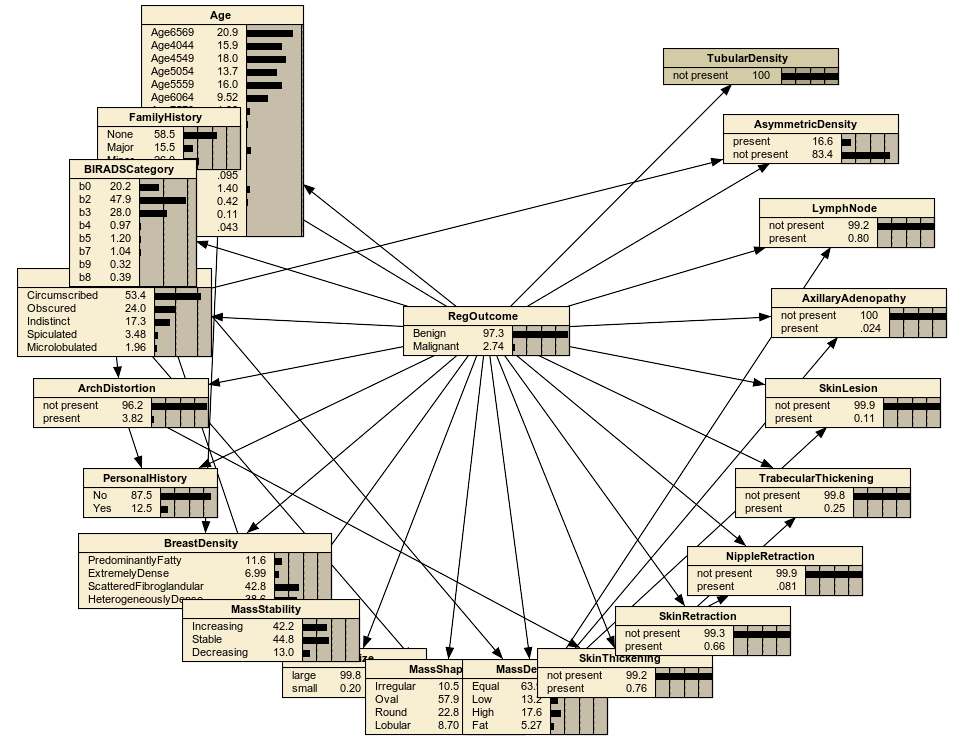
\includegraphics[width=\linewidth]{mass_net.png}
	\caption{The learned TAN model linking descriptors to malignancy}
	\label{fig:mass_net}
\end{figure}


\clearpage
\begin{figure}
\centering
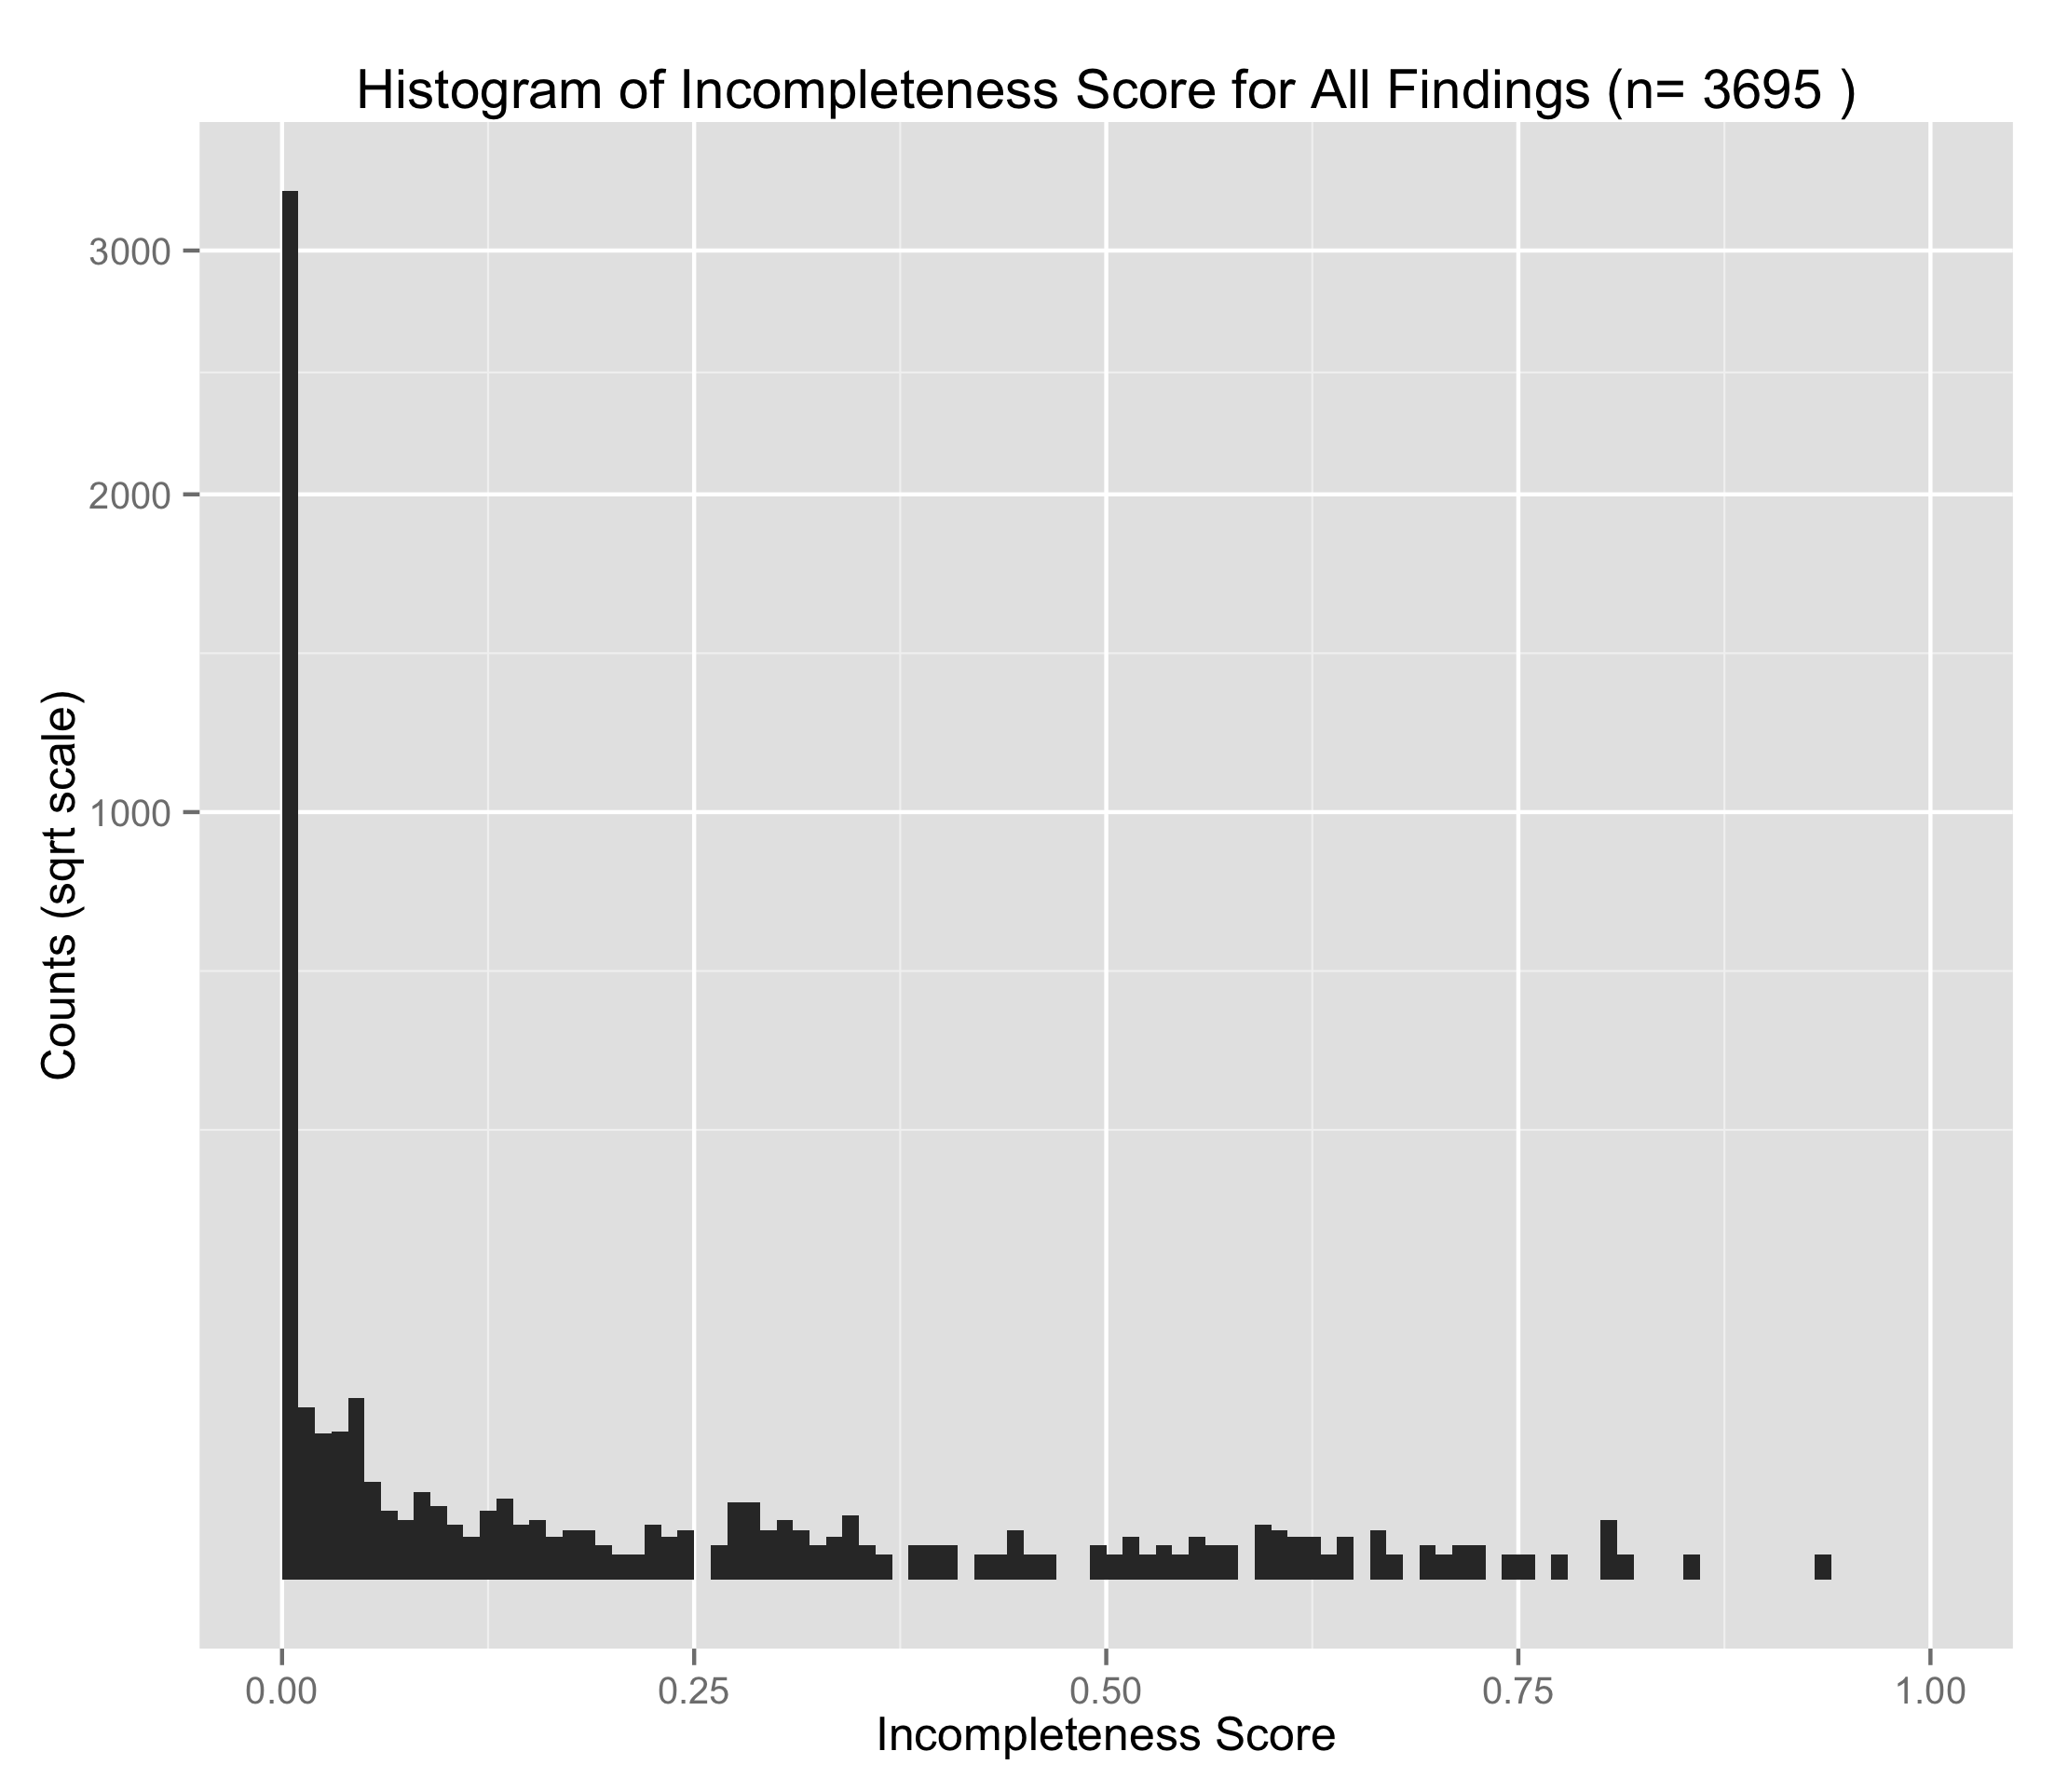
\includegraphics[width=\linewidth]{incompleteness_score_hist_all.png}
\caption{Histogram of all incompleteness scores in the test data set}
\label{fig:incompleteness_score_hist_all}
\end{figure}


\clearpage
In order to verify that the incompleteness score can be used to predict mammographic error, I plotted its histogram and density estimate stratified by radiological predictive categories: true negative (TN), false negative (FN), true positive (TP), and false positive (FP) [figure \ref{fig:incompleteness_score_hist_confmat}]. The graphs show that there are a large number of false positive and false negative cases that have non-zero incompleteness scores. Intuitively, this shows that incomplete reports have a higher likelihood of containing errors. The mean incompleteness score for erroneous cases ($FP \cup FN$) was \textbf{0.0720} while the mean incompleteness score for correct ($TP \cup TN$) cases was \textbf{0.0079}, an order of magnitude smaller. The difference between error and non-error incompleteness scores was statistically significant ($p < 2.2*10^{-16}$).

\begin{figure}
\centering
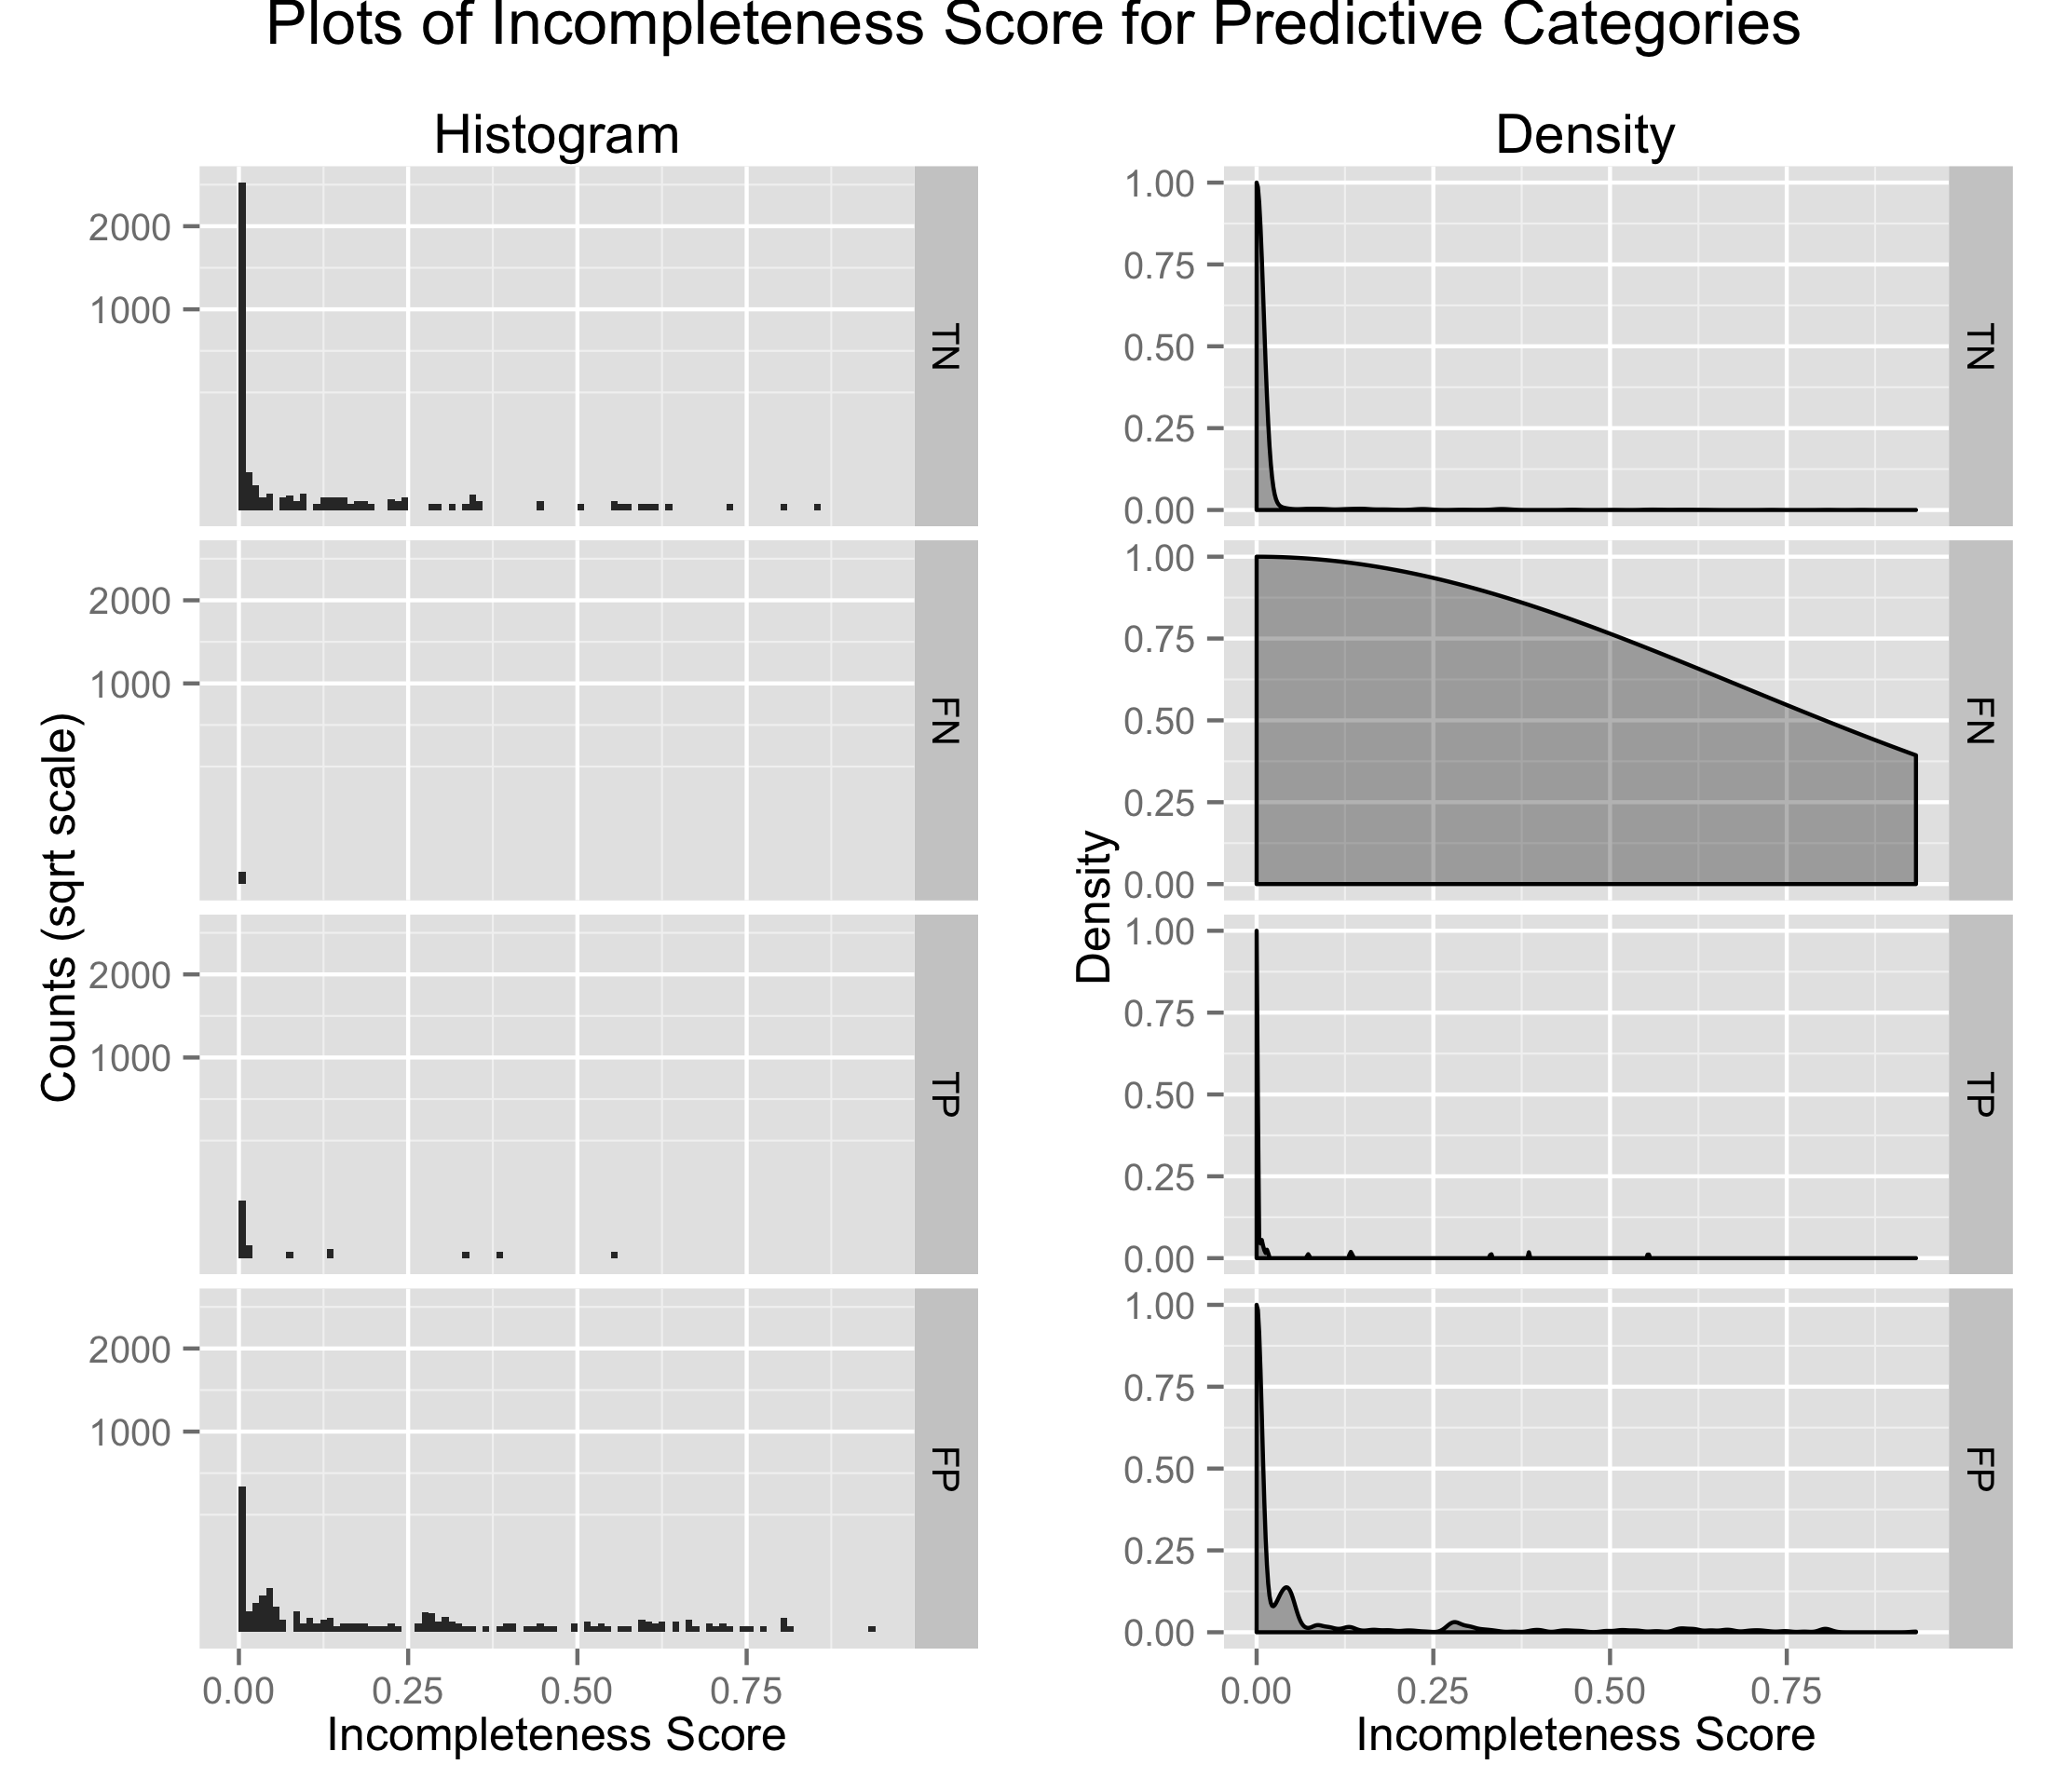
\includegraphics[width=\linewidth]{incompleteness_score_hist_confmat.png}
\caption[Incompleteness scores stratified by confusion matrix]{Plots of the histogram and density of incompleteness scores, stratified by radiologist performance on their respective cases. True Negative (TN) findings have the lowest incompleteness scores (indicating they are most complete) while false positive (FP) findings have higher incompleteness scores (indicating less completely reported findings). Joining (TN,TP) and (FP,FN), I can compare cases that were correctly assessed to cases with errors. Note that the false negative density graph has a nearly uniform distribution. This is an artifact due to the small amount of false negatives in the data set that skew density estimation.}
\label{fig:incompleteness_score_hist_confmat}
\end{figure}


An issue with this data is that there are a small number of false negative findings compared to false positive findings. This could skew results since positive findings may contain descriptors more prone to noise in the model. To account for this, I compared false positive to true positive results since both groups would have similar descriptors. The analysis showed that they were still statistically significantly different ($p<0.0026$).

\clearpage

I then tested how well the incompleteness score could predict error in mammography reading. Figure \ref{fig:incompleteness_rad_improvement} shows several performance metrics for different cutoffs of the incompleteness score. The maximal accuracy with respect to cutoffs was 0.826 at a cutoff of 0.018. This means that < 1.8\% probability of changing decisions when given new information should warrant describing more observations. The precision associated with this cutoff was 0.713 meaning 71.3\% of cases classified as errors via the incompleteness score with cutoff 0.018 will actually be errors. Finally, I measured the percentage reduction in total mammography error if each error marked for revision was corrected. Using the given cutoff, we saw a potential 21.7\% decrease in total errors.

\begin{figure}
\centering
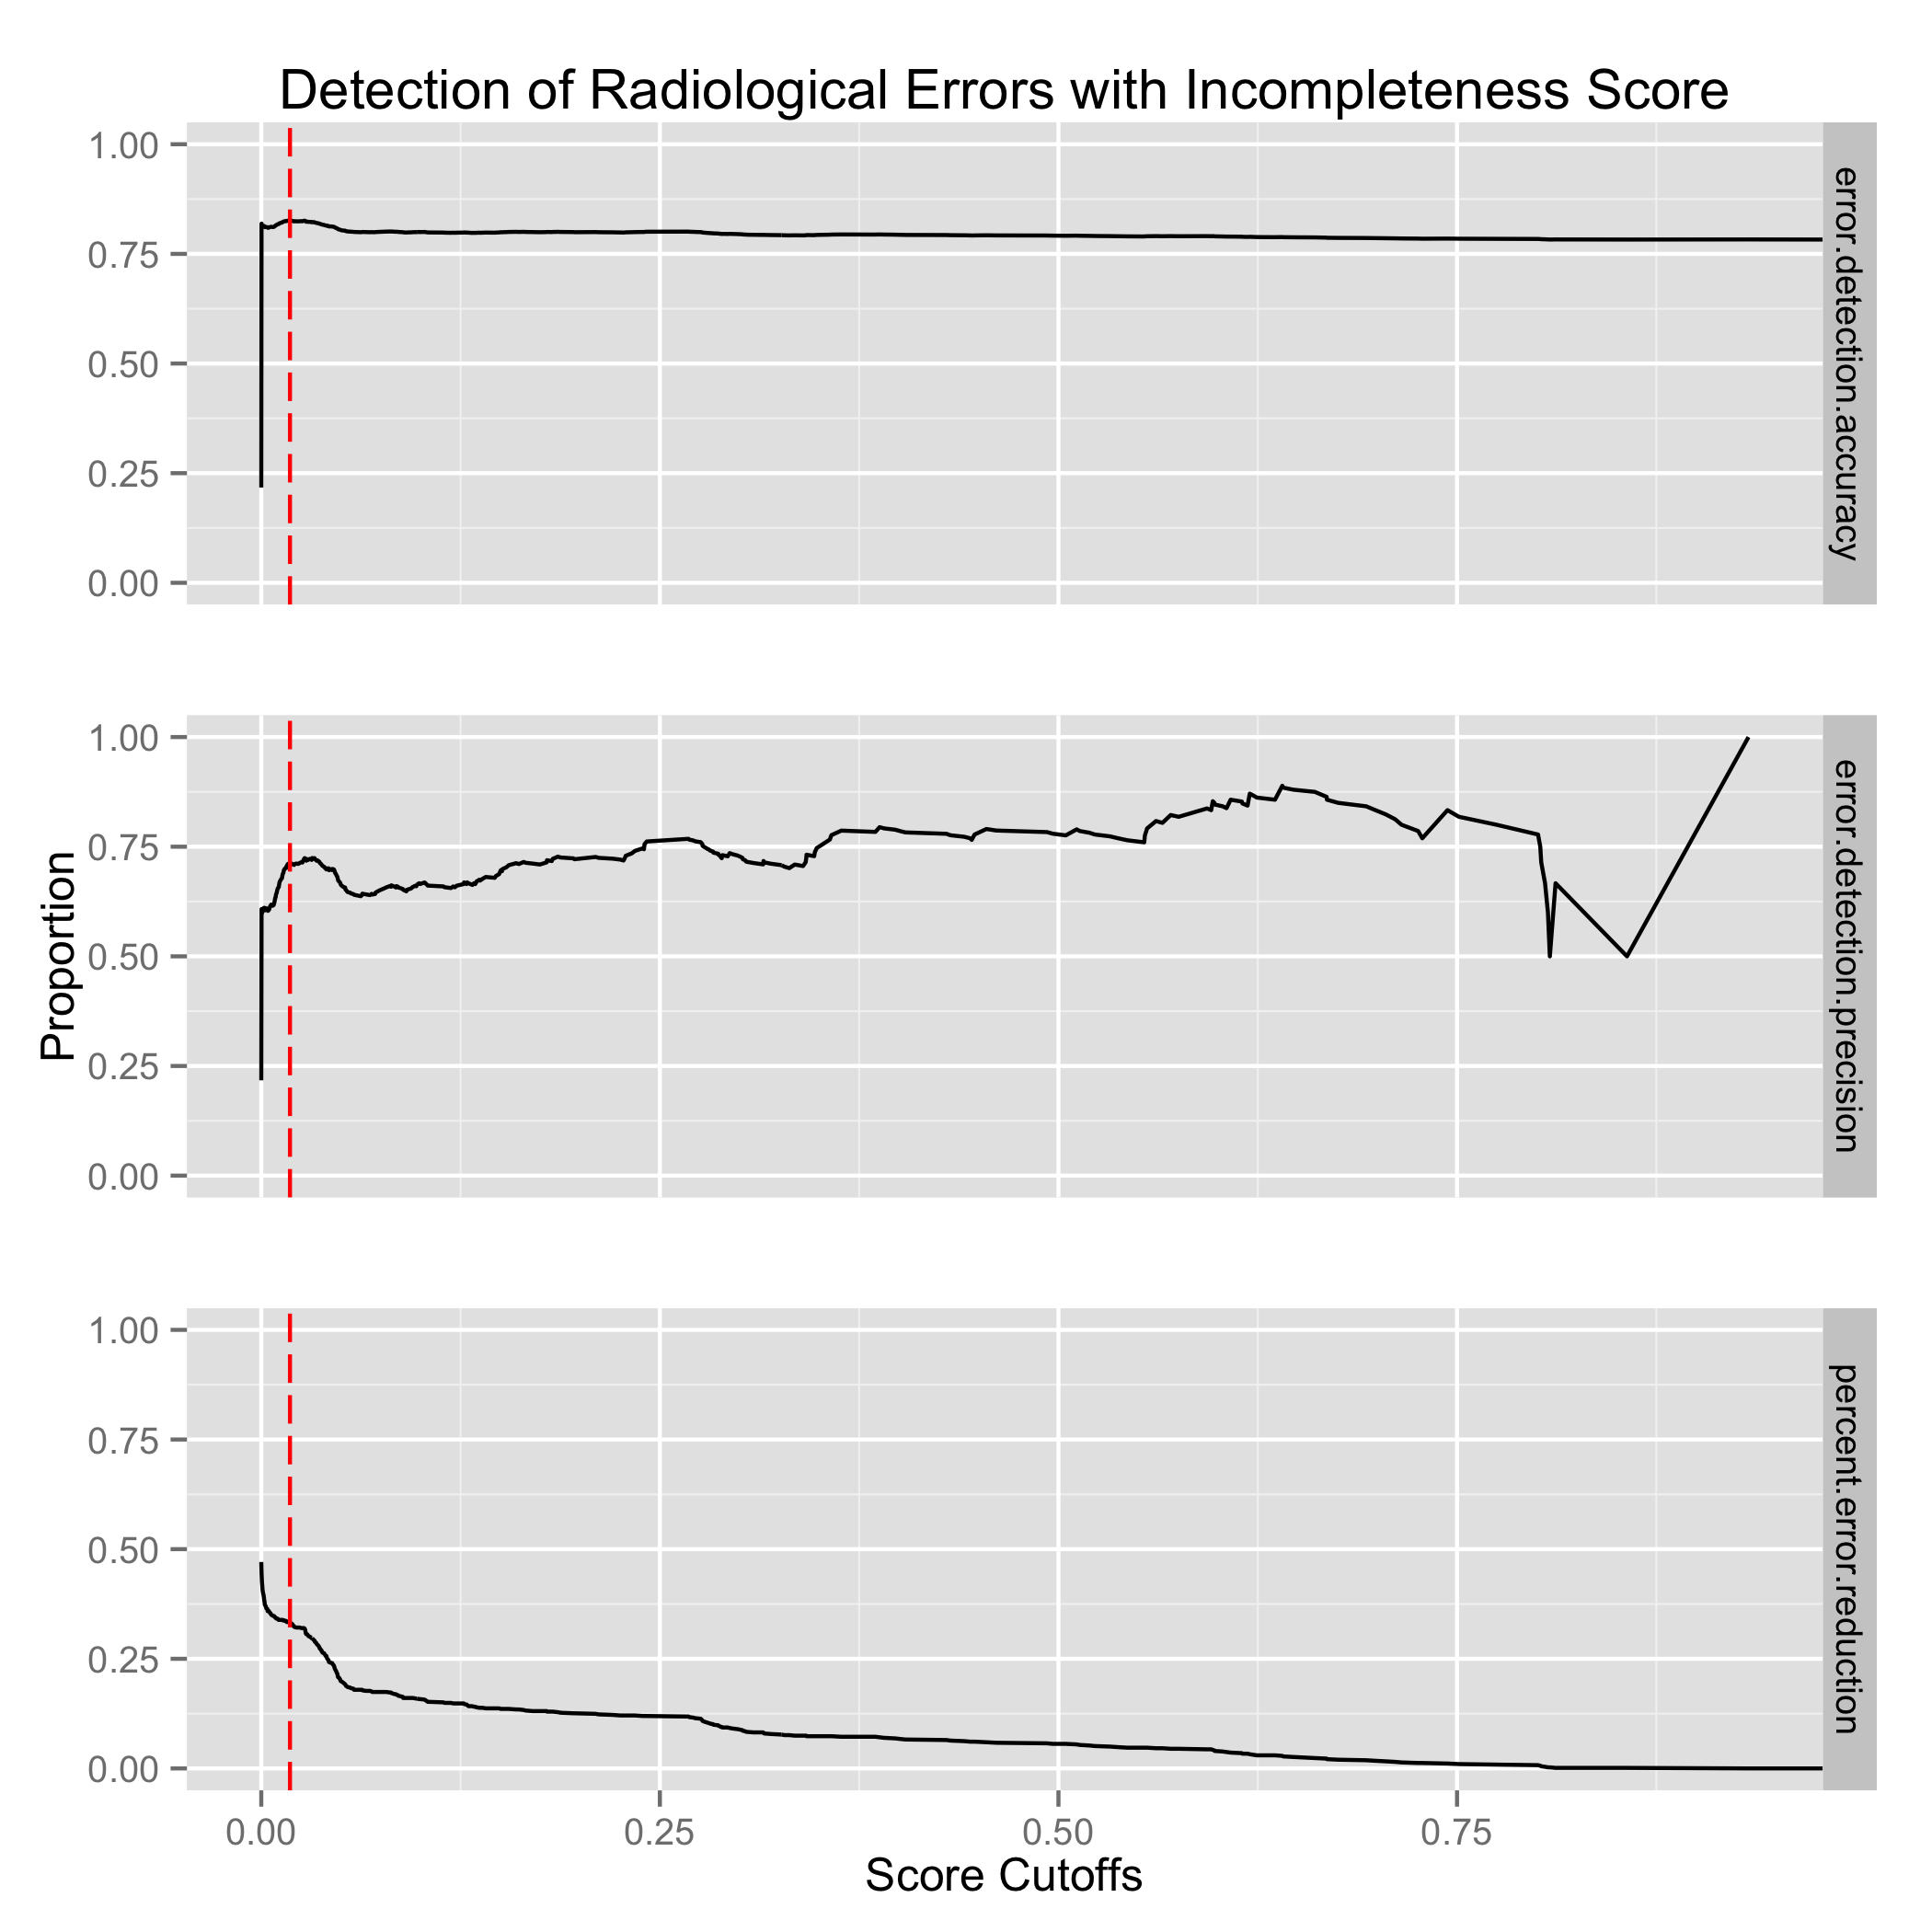
\includegraphics[width=\linewidth]{incompleteness_rad_improvement.png}
\caption[Radiological improvement with incompleteness scores]{Improvement in radiological performance for difference incompleteness cutoffs. First row shows the incompleteness score accuracy in predicting radiological errors. Second row shows incompleteness score positive predictive value in predicting error. Third row shows the percent reduction in error if identifying error at the specified cutoff. The red-dotted line shows the cutoff point that maximizes error classification accuracy (first panel).}
\label{fig:incompleteness_rad_improvement}
\end{figure}

\clearpage

\section{Discussion}
I described a method to quantify incompleteness in a mammography report. I then presented an algorithm to measure this value in a computationally tractable manner. Finally, I showed that this incompleteness score is a strong indicator of errors in mammography interpretation. Implementation of this metric during mammography reporting time could provide a useful real-time feedback to radiologists to indicate possible errors.

\subsection{The benefits of complete reports}
Reporting in mammography is a labor intensive but critically important task for results communication. Though there is pressure for radiologists to produce their efforts efficiently, we show that poor report quality (measured by our incompleteness score) is a marker for interpretation errors. This result might stem from a few different causes. The causal explanation is that poor interpretation leads to poor reports. In this case, a radiologist might have not seen a relevant descriptor in the image or neglected to highlight its importance. Another possibility is that incomplete reporting is a function of available time. When required to read large volumes of images, speed may decrease accuracy. In this case, a practitioner producing brief or incomplete reports may also be spending less time interpreting the image. A third possibility is that the process of reporting improves diagnosis by requiring radiologists to reason about their diagnosis. Thus, individuals who do not spend as much time on their reports do not go through the same formal thinking process. For future work, we will consult breast imaging radiologists on cases that were correctly classified as erroneous to see if humans can also identify when poor reporting leads to mis-diagnosis. If this is the case, we can begin to discover reporting practices that reduce error rates.

\subsection{Limitations of this study}
Though the system shows promising results with regards to predicting radiological errors, it does have some shortcomings. The use of an approximate algorithm to estimate the incompleteness score allows for some degree of error. I correct for this by using a large number of samples with respect to the number of hidden variables, but unfortunately, it is difficult to empirically evaluate my system as calculating the exact incompleteness score is prohibitively expensive with regards to computational time. For future work, I will evaluate alternative approaches for measuring incompleteness. Another issue with our system is that it does not actually correct the errors in interpretation or give any constructive feedback. So although the system can potentially reduce the amount of errors by  ~20\%, I have not shown which of these reports would actually be corrected. We address this topic in the next chapter. This study was designed to be descriptive rather than predictive, so I did not measure classification results with an optimal cutoff in a third held-out test set. Thus, the results will be overly-optimistic in terms of error-prediction. In the future, I plan to implement our algorithm on faster cluster computers, which will allow me to perform a thorough cross-validation analysis to obtain better accuracy measurements. Finally, this system hinges on an accurate, generative probabilistic classification model. We leverage the success of previous work \cite{Burnside:2009br} to do this analysis, but the availability of such systems may be limited in other domains.

\subsection{Extension to other domains}
This methodology could be extend to any domain that uses expensive information to make threshold-based decisions. This system requires is a generative model linking descriptors to diagnosis and a method to sample from this model. Construction of such models is extremely difficult without large, high quality data sets that have ground-truth. Efforts to leverage hospital data via learning healthcare systems should help create more fertile domains for creating these models. That being said, once proper decision support models are learned, it is straightforward to implement this in any medical domain where testing can be a costly and/or risky task. Not only can this method improve diagnostic accuracy, but it inherently rewards good, thorough reporting practices. This is beneficial for patients and researchers alike.

\clearpage
\chapter{Providing Feedback to Radiologists}

\section{Feedback: Introduction}
\subimport{}{feedback_intro}
\clearpage

\section{Feedback: Method}
\subimport{}{feedback_method}
\clearpage

\section{Feedback: Experiment Design}
\subimport{}{feedback_experiment_design}
\clearpage

\section{Feedback: Results}
\subimport{}{feedback_results}
\clearpage

\section{Feedback: Discussion}
\subimport{}{feedback_discussion}
\chapter{Conclusions}

\section{Informatics Contribution}
\subimport{}{informatics_contribution}
\clearpage

\section{Biomedical Contribution}
\subimport{}{biomedical_contribution}
\clearpage

\section{Proposed Work}
\subimport{}{proposed_work}


%---------------------------------------------------------------------------------------------------
% Appendices. Each must begin with: \chapter{myAppendixTitle}.

%\appendix
%\include{appendixFN}

%---------------------------------------------------------------------------------------------------
% Bibliography and dismount.
\bibliography{bib/bibtex_lib_dec_2015.bib}		% full path to .bib (bibtex file)
\end{document}
